\chapter{Regularization Methods\label{cha:regularization}}
During the discussion of \vref{eq:optGoal} we neglected the regularization
operator \(\mathcal{S} \from \mathbb{R}^d \to \mathbb{R}\).
This chapter starts with a short introduction to statistical regularization
theory and then compares two groups of regularization methods:
Tikhonov regularization and sparse regularization.

\section{Regularization Theory}
Regularization helps us to train models that not only fit the data, but also generalize well.
To understand regularization, it is helpful to decompose our error functional.
Our model assumes, that there is a relation between the predictors
(\(\bm{x}\)) and the target variable (\(y\)) that can be expressed as
\begin{equation*}
  y = f(\bm{x}) + \varepsilon,\, \varepsilon \sim \mathcal{N}(0, \sigma^2),
\end{equation*}
where \(f(\bm{x})\) is the function we want to approximate.
Consider the expected prediction error at a point \(x\)~\cite{esl}:
\begin{align}
  \label{eq:bias-variance}
  \text{Pred.~error}\left( x \right) = \Exp \left[ \left(y - \hat{f}(x) \right)^2 \right] &=
              \Bias\left[\hat{f}(x) \right]^2 + \Var\left[\hat{f}(x)\right] + \sigma^2 \\
  \Bias \left[ \hat{f} (x) \right] &= \Exp \left[\hat{f}(x)\right] - f(x), \nonumber \\
  \Var \left[ \hat{f} (x) \right] &= \Exp \left[ \hat{f}(x) - \Exp \left[ \hat{f}(x) \right]^2 \right] \nonumber,
\end{align}
where \(\hat{f}(x)\) denotes our approximation of the real function \(f(\bm{x})\).
\sidetitle{Bias-Variance trade-off}
We call \cref{eq:bias-variance} the bias-variance trade-off.
This equation splits the error into three different parts:
\begin{description}
\item[Bias] is the error caused by assumptions the model makes,
\item[variance] is the error caused by noise in the training data and the
\item[irreduziable error (\(\sigma\))] is the error caused by noise that is inherent to the relation between the predictors and the target variable.
\end{description}

Following the principle of \emph{Occam's razor} --- parsimonious models are better --- all regularization models penalize complexity.
Using regularization leads to smaller and simpler models, which increases the bias.
Of course, increasing this part of the error term makes no sense, if we would not get a payoff.
Regularization decreases the variance, thus making our model more robust to the possibly noisy data.
In this chapter we consider regularization methods that have both a scaling parameter, that controls the strength of our assumptions, and (sometimes) parameters, that we use to modify the kind of our assumptions.
We call the parameter that controls the regularization strength \(\lambda\).

\sidetitle{Finding \(\lambda\)}
The choice of this parameter is important:
If we increase \(\lambda\), we exchange more bias for variance.
This is why \cref{eq:bias-variance} implies a trade-off --- we cannot eat the cake and have it too!
We usually find the ideal \(\lambda\) by a more-or-less intelligent trial and error process.
To do this, we train a predictor for each \(\lambda\) we want to consider on a subset of our data (called the training set), and test its performance using either cross-validation or a separate (holdout) validation set. 

\sidetitle{Prior Information}
Another way to reason about regularization is that it allow us to encode our
assumptions directly into the training process.
Many regularization methods --- and all mentioned in this chapter --- can be
viewed from a Bayesian perspective, which gives an intuitive explanation of the
effect of our assumptions.

The choice of the regularization functional is crucial.
We do not know which one performs best without training a model.
Sometimes we can encode knowledge about the dataset structure, but this is often
quite difficult.
We try to present heuristics for this during the following sections, when applicable.

In this chapter we will compare multiple choices and evaluate their effectiveness.
Each method encodes different assumptions, but all have in common that they decrease
our model complexity.

\section{Tikhonov Regularization}
\subsection{Theory}
Instead of solving an unconstrained minimization problem, we solve the following
problem:
\begin{align}\label{eq:tik-constrained}
 \text{minimize} \quad &
 \left\Vert  \bm{\Phi} \bm{\alpha} - \bm{y}  \right\Vert_2^2 \nonumber \\
\text{subject to} \quad &  \Vert \bm{\Gamma} \bm{\alpha}  \Vert_2 \leq l,
\end{align}
for a certain constant \(l\) and a linear operator \(\bm{\Gamma}\). 
By doing this we force our scaled weights to lie inside a \(d\)-dimensional sphere with a diameter of length \(l\).
To get a more convenient representation of~\cref{eq:tik-constrained} we use Lagrange multipliers to cast it into the equivalent Lagrangian form.
We then recover our goal~(\ref{eq:optGoal}) with
\begin{equation}\label{eq:tik-langrangian}
\mathcal{S} = \lambda \Vert \bm{\Gamma} \bm{\alpha} \Vert_2^2
\end{equation}
as the smoothness functional.
This method is called Tikhonov regularization.
There is an one-to-one correspondence between \(l\) in~\cref{eq:tik-constrained} and \(\lambda\) in~\cref{eq:tik-langrangian}.
Both variables determine the constraints.
Tikhonov regularization fits into a Bayesian framework.
We can interpret it as a multivariate-Gaussian prior on the weights with zero mean and covariance matrix \(\bm{\Gamma}^{-1}\)~\cite{stat-inverse}.
The weights are therefore distributed as follows
\begin{equation*}
\alpha \sim \mathcal{N} (0, \bm{\Gamma}^{-1}).
\end{equation*}

A common choice for \(\Gamma\) is the identity matrix as proposed in~\cite{spatAdaptGrid}.
This corresponds to a penalty on the summed squared values of the weights.
It is a Gaussian prior with the identity matrix as its covariance matrix.
In statistics, this method is called ridge regression.

\sidetitle{Diagonal Matrix}
This method assumes that all weights are distributed with the same variance.
Luckily, we can do better for the sparse grid methods.
Following the assumption of \vref{eq:coefficients-h2mix}, we can express every
function \(f \in H_2^{\text{mix}}\) as a weighted sum of basis functions.
For these functions the following upper bound on the hierarchical coefficients \(\alpha_{\bm{l, i}}\) holds:
\begin{align}\label{eq:weights-bound}
  \vert \alpha_{\bm{l, i}} \vert &\leq 2^{-d -2 \vert \bm{l} \vert_1} \cdot \Vert D^{\bm{2}} f \Vert_{\infty} \\
                              &\in \BigO \left( 2^{-2 \vert \bm{l} \vert_1} \right)
\end{align}
where the differential operator norm only depends on the function \(f\) and neither on the dimension nor the level of the basis functions~\cite{bungartzSparse}.
Because the dimension is constant for a given grid, it is treated as a constant.

This fact can be used to implement a regularization method that is better suited for functions in \(H^2_\text{mix}\).
We impose an improved prior on the weights using Tikhonov regularization
with the matrix
\begin{equation}\label{eq:diagonal-prior}
\bm{\Gamma}_{i,i}^{1} = c^{\vert l \vert_1 - d},
\end{equation}
with a constant \(c\).
For \(c = 4\) this corresponds to a prior on the variance of the weights that is identical to the upper bound given by \cref{eq:weights-bound} up to a multiplicative constant.
A different \(c\) can be used as well, we can either treat \(c\) as an inherent property of the method or as an additional hyper-parameter.
We use the dimension \(d\) as a normalizing factor, this way the prior
corresponds to the series \((1, \nicefrac{1}{4}, \nicefrac{1}{16}, \ldots)\).
The resulting series is depicted in \vref{fig:diagonal} for a two dimensional grid.

\begin{figure}[htb]
  \centering
  \begin{minipage}[c]{0.6\textwidth}
    \centering
    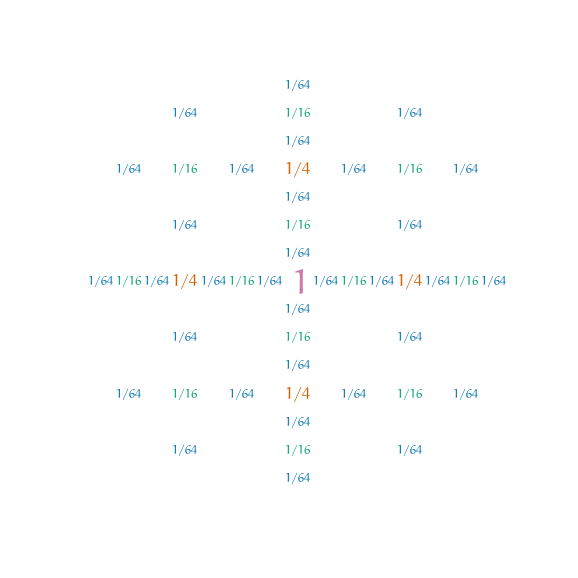
\includegraphics[width=1\textwidth]{diagonal}
  \end{minipage}\hfill
  \begin{minipage}[c]{0.4\textwidth}
\caption[Diagonal Regularization]{
This figure shows the prior generated by \cref{eq:diagonal-prior} for a two
dimensional grid with level two. Each number is centered on a grid point and
corresponds to the prior for that particular weight.
}\label{fig:diagonal}
  \end{minipage}
\end{figure}

\FloatBarrier{}

\subsection{Implementation}
\todo{Maybe create a class diagram for the implementation of the DiagonalMatrix?}
Each regularization method that can be used with the conjugated gradient solver
is implemented in the \textsc{sgpp} by specialising the super class
OperationMatrix that offers a method called ``mult'' which accepts a weight
vector and returns a scaled version of the weights.
The OperationMatrix for the standard ridge regularization returns its input
weights unchanged.

The DiagonalMatrix implementation has multiplies each input weight with the
corresponding inverse prior.
We calculate the multiplier for each weight during the first call of the
multiplication method and cache it until the grid size changes.
This means that we only need to perform this calculation once per refinement
step.
We determine the multiplier for each grid point by simple iterating over all
existing grid points and save the reciprocal of the result of \cref{eq:diagonal-prior}.

\subsection{Results \textit{\&} Discussion}
To prove the effectiveness of our method, we first show empirically that \cref{eq:weights-bound} holds for a simple function in \(H^2_{\text{mix}}\).
We then present results that indicate that our proposed regularization functional shows improved results for an artificial dataset, for that the upper bound for the surpluses holds by construction.
Finally we show benchmark results for two real-world datasets, comparing the identity matrix with the diagonal operator.

\begin{figure}[ht]
  \centering
    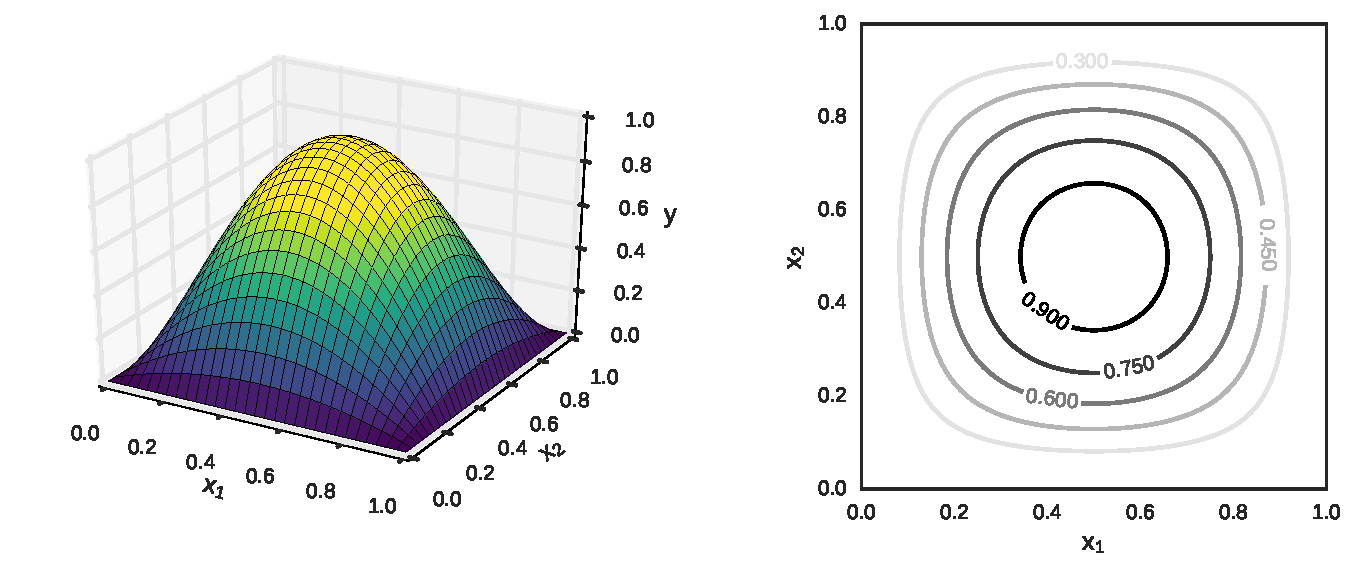
\includegraphics[width=1\textwidth]{parabola_contour}
  \caption{Contour and surface plot of the inverse parabola function.}
\end{figure}
Consider the inverse parabola \(y^P(x_1, x_2)\) given by
\begin{equation}\label{eq:inverse-parabola}
  y^p(x_1, x_2) = 16x(1-x)y(1-y).
\end{equation}
\sidetitle{Inverse Parabola}
\todo{Cite inverse parabola?}
We created a two dimensional grid with standard linear basis functions and an arbitrary level.
Without loss of generality we chose a grid with level three that has 17 grid
points.
The dataset was then created by setting each \(x_1, x_2\) equal to the coordinates of one grid point each, \(y\) is then calculated using \cref{eq:inverse-parabola}.
The sparse grid regression model trained on this dataset and the aforementioned
grid was able to recover the data perfectly, with a mean squared error smaller than the machine epsilon. More interestingly, the calculated weights were identical to our prior.
While this does not prove that this prior holds, it is a simple example for this construction.

But does our prior improve the results for a function, when we include our prior
knowledge about the weights bound?
\sidetitle{Recovering Weights}
To test this hypothesis, we constructed another artificial dataset.
We first created a two dimensional sparse grid learner with level 3 and sampled its weights from the normal distribution, such that the distribution of the surpluses was given by \(\bm{\alpha} \sim \mathcal{N}(0, \bm{\Gamma}^{-1})\).
That corresponds directly to the multidimensional Gaussian prior, as described by \cref{eq:diagonal-prior}.
Let \(\bm{X} \in \mathbb{R}^{n \times 2}\) be our matrix, where each row is drawn from a two-dimensional uniform distribution.
We then created our target vector \(\bm{y}\) by predicting the result of
\(\bm{X}\) using the constructed model.
Right now, this gives a trivial regression problem and to show the effect of our
proposed regularization method, we need to add some noise to \(y\).
Let \(\sigma\) denote the standard deviation of \(y\).
We then crafted different variants of our dataset by adding normal noise to the
target variable with mean zero and standard deviation \(s \sigma\), for some
values of \(s\).
The signal-to-noise-ratio (\textsc{snr}) of the modified target is then given by \(1/s\).

\todo{Use scientific notation for \(\lambda\).}
\begin{table}[htb]
\centering
\begin{tabular}[c]{S[table-format=2.1]S[table-format=1.1]S[table-format=2.6]S[table-format=2.6]S[table-format=2.6]S[table-format=2.6]}
  \toprule \multicolumn{1}{r}{SNR}
& \multicolumn{1}{r}{Exponent Base}
& \multicolumn{1}{r}{\(\lambda\)}
& \multicolumn{1}{r}{Weights-RMSE}
& \multicolumn{1}{r}{CV-RMSE}
& \multicolumn{1}{r}{\(\sigma_\text{noise}\)}
\\\midrule
0.5 & 4.5 & 0.002442 & 0.109284 & 2.159250 & 2.100775\\
1.0 & 6.5 & 0.000256 & 0.095696 & 1.083762 & 1.050387\\
2.0 & 4.5 & 0.000146 & 0.080263 & 0.545097 & 0.525194\\
4.0 & 4.0 & 0.000047 & 0.062738 & 0.274558 & 0.262597\\
\bottomrule
\end{tabular}
\caption[Best exponent bases for diagonal test dataset.]{
  This table shows the best exponent base~\(\times\,\lambda\) combination.
The first half of the table presents the best results determined by the
weights-\textsc{rmse} metric, the second half the best results ordered by the cross
validation prediction error.}\label{fig:diagonal-testdata}
\end{table}

We performed a grid search\footnote{
We used a monte-carlo cross-validation method with ten iterations and
a 9:1 train-validation split for this experiment, in contrast to the usual
10-Fold method to compare the different estimators.
} for sparse grid estimators, testing on a grid
consisting of different choices for \(\lambda\) and the exponent bases in the
interval \([2, 10]\) with stepsize 0.5.
The results for the best parameters can be seen in \cref{fig:diagonal-testdata}.
Note that we archived the best cross validations errors with exponent bases
that are close to four, with one outlier.
The regularization parameter \(\lambda\) and the \textsc{rmse} for the weights
decreases for a higher \textsc{snr}, as expected.
All results are close to the theoretical optimal error, given by the variance of
the noise.
Those results indicate, that our proposed regularization method improves performance for a dataset, which can be approximated by a model with surpluses that follow the upper bound.

\sidetitle{Concrete dataset}
So far we have only seen examples for artificial datasets which adhere to our assumptions by construction.
We now introduce our first real-world dataset, the concrete dataset.
For this dataset our goal is to predict the compressive strength of concrete,
using the recipe and the age in days of its mixture.
The recipe consists of seven quantitative predictors, all given in the unit
kilogram per thousand liters.
Concrete consists of the ingredients cement, blast furnace slag, fly ash,
water, super-plasticizer, coarse aggregate, and fine aggregate.
It was donated to the \textsc{uci} machine learning
repository~\cite{datasets-uci} by \citeauthor{datasets-concrete} and was first
published in their paper~\cite{datasets-concrete}.
The dataset consists of 1030 instances altogether.
We split the data and used 80\% for training, and the other 20\% solely as
testing data.

We performed a grid search using a learner with level 4 for the diagonal
regularization with fixed exponent bases \(c = 4\), and \(c = 1\), which is equal
to the standard ridge regularization method.
Each learner performed five adaptivity steps, refining five grid points during
each step.
The performance of each estimator was estimated using a standard 10-fold cross
validation procedure.

\begin{figure}[htb]
  \centering
  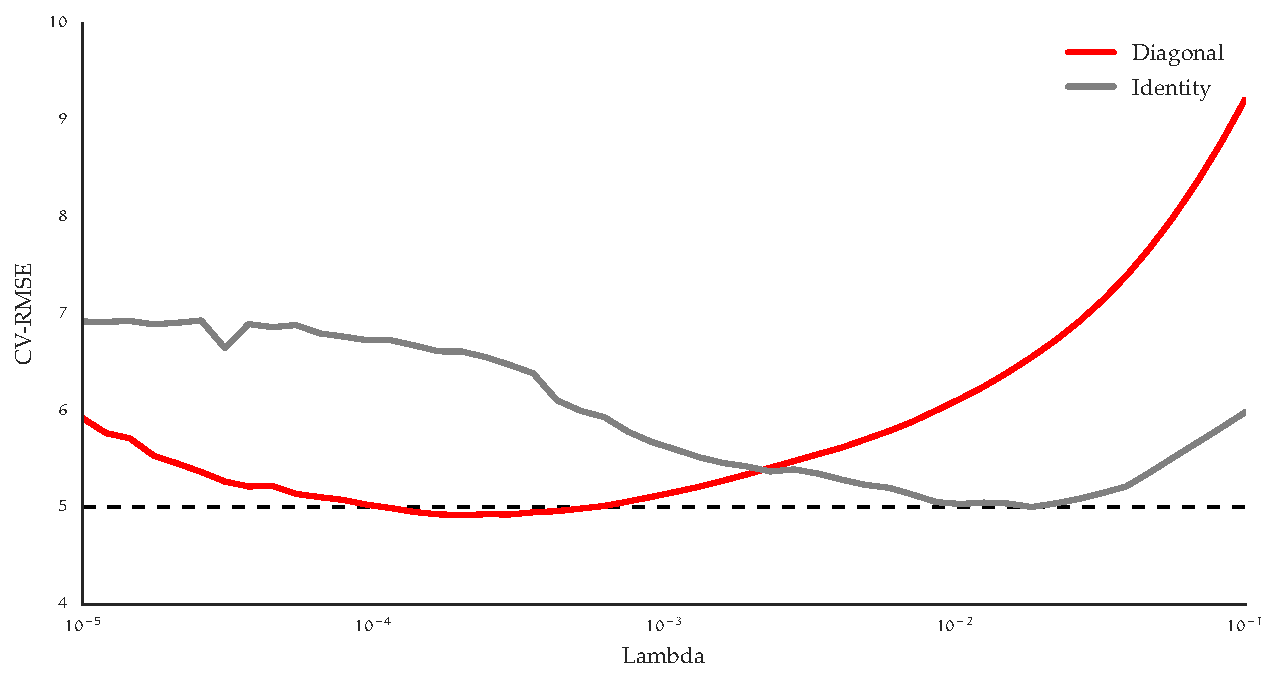
\includegraphics[width=\textwidth]{tikhonov_concrete_l4}
  \caption{This figure presents the obtained results for the concrete dataset
    obtained with estimators with level four.}
  \label{fig:tikhonov-concrete-l4}
\end{figure}

The results are shown in \cref{fig:tikhonov-concrete-l4}.
We can see that our method results in better results than the identity
regularization, although the difference between the two methods was small.
\FloatBarrier{}
\sidetitle{Power Plant Dataset}
\begin{figure}[htb]
  \centering
  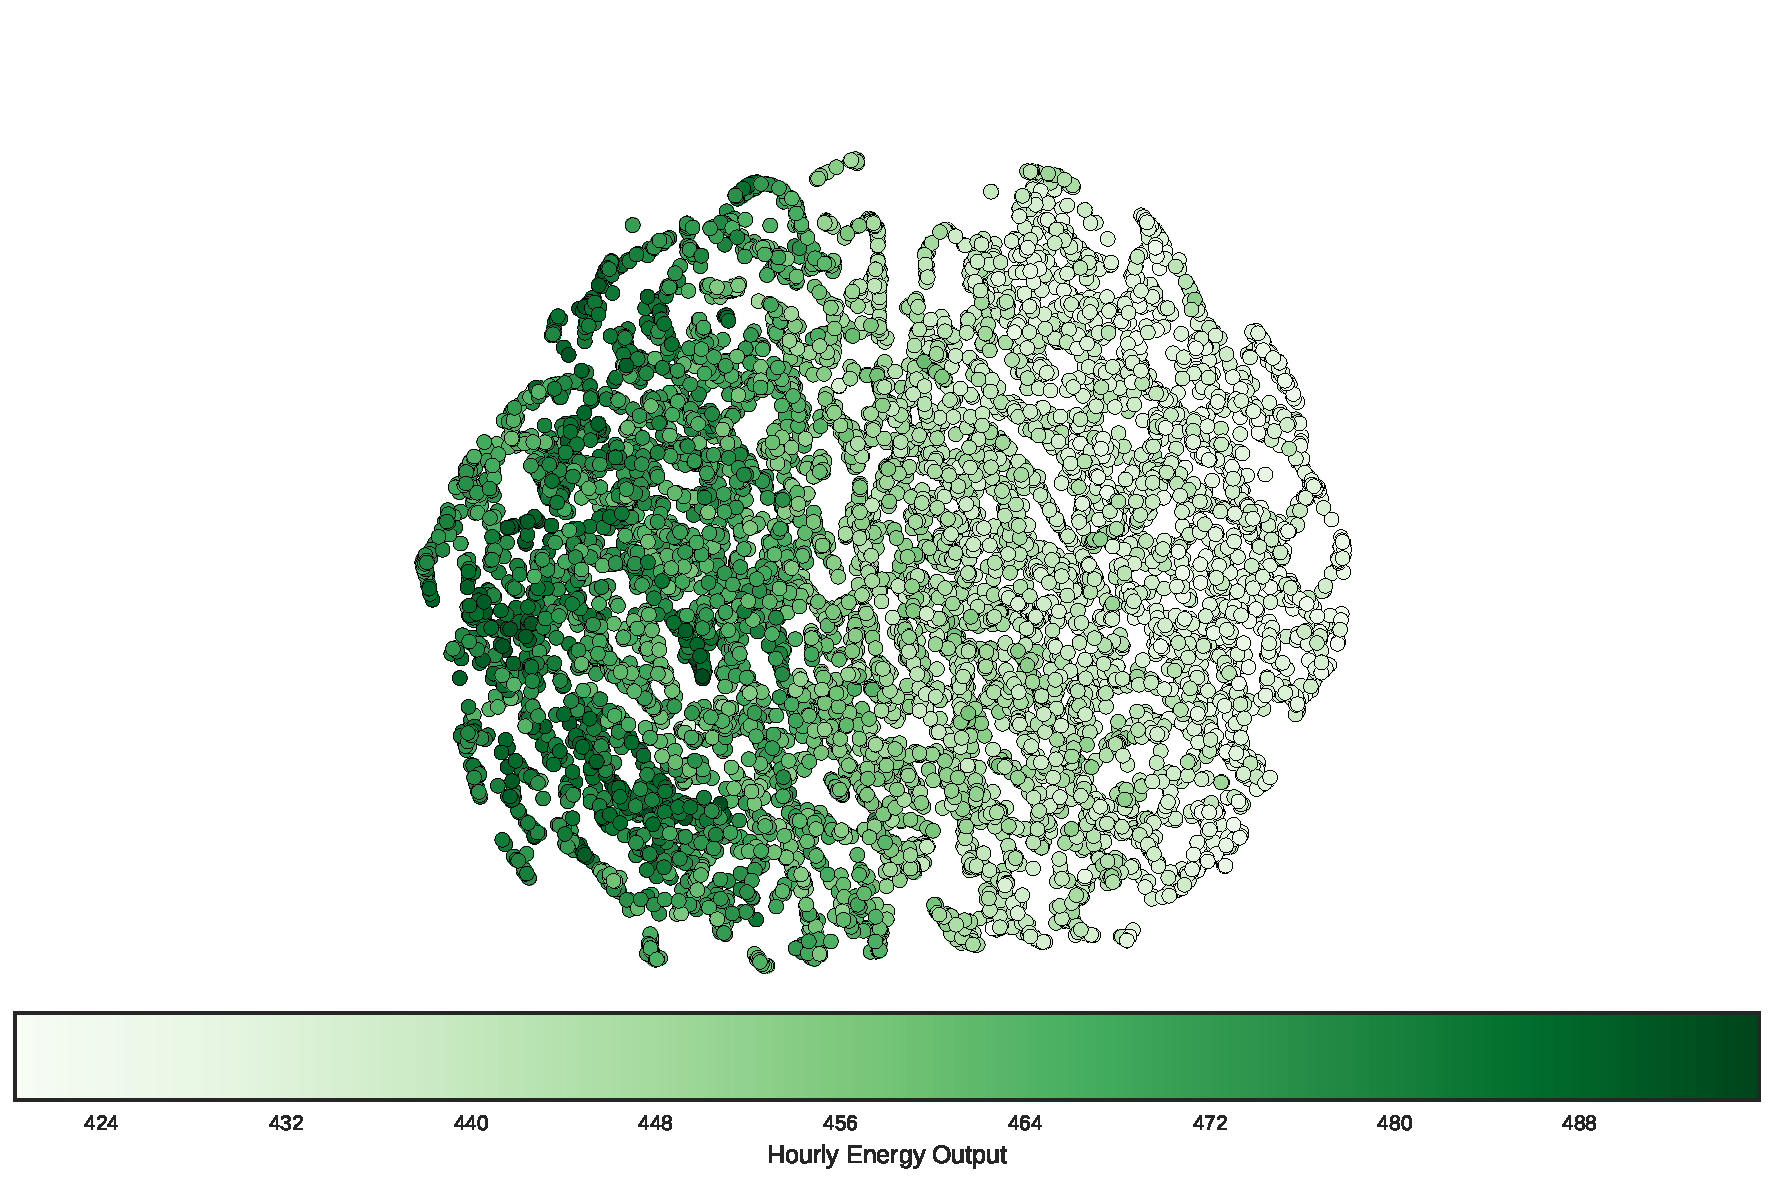
\includegraphics[width=\textwidth]{tsne_power_plant}
  \caption[\textsc{t-sne} plot for the power plant dataset]{
This figure shows the power plant dataset. This visualization is generated using the T-distributed stochastic neighbor embedding (\textsc{t-sne}) algorithm. Data points that are close to each other in the
  original, multi-dimensional dataset are also close in this two-dimensional
  representation. The target values are not considered for this calculation, they
are only used to determine the color of the points. The axes contain no useful
information and are therefore omitted.
}
  \label{fig:tsne-power-plant}
\end{figure}

We also tested the performance for the power plant dataset, for which a visualization is given by \cref{fig:tsne-power-plant}.
The target variable of this dataset is the hourly energy output for a combined
cycle power plant.
To predict this target, we use the temperature, the ambient pressure, the
relative humidity, and the exhaust vacuum as predictors.
This dataset appeared first in~\cite{datasets-powerplant} and was donated to the
\textsc{uci} machine learning repository~\cite{datasets-uci} by \citeauthor{datasets-powerplant}.
It consists of 9568 instances, which were split into a training and testing
dataset at a ratio of 8:2.

We then performed a grid search over an grid of lambdas in the interval
\([10^{-10}, 10^{-1}]\) for learners with level 5, again using ten-fold cross validation.
The grids were refined five times, refining three points for each adaptivity step.
The results can be seen in \cref{fig:tikhonov-power-plant-l5}.
Note that this figure only shows the results in a small interval, all values of
\(\lambda\) that were larger than the values shown resulted in far larger
errors.
Again, we can see that the diagonal regularization was able to archive better
results by a small margin.

We can conclude from these results, that the diagonal regularization method is
able to result in better outcomes if the datasets adhere to the assumptions of
the method.
The tests on real-world datasets showed, that our method is a solid alternative
to the standard ridge regularization functional, increasing the performance by a
small margin for a negligible additional performance cost.

\begin{figure}[htb]
  \centering
  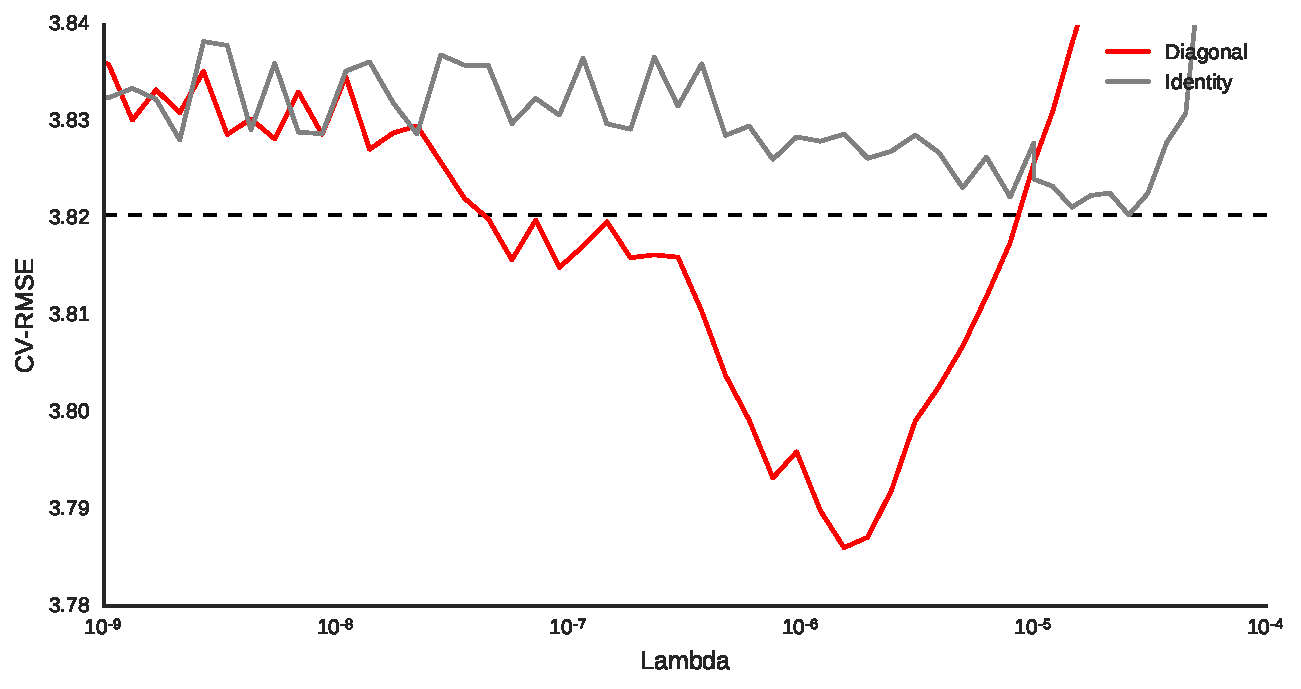
\includegraphics[width=\textwidth]{tikhonov_power_plant_l5}
  \caption{This figure compares the diagonal regularization method with the
    standard ridge functional for the power plant dataset for different learners
  with level five.}
  \label{fig:tikhonov-power-plant-l5}
\end{figure}
\FloatBarrier{}
\section{Sparse Regularization}
We have seen different variations of Tikhonov regularization.
All regularization methods so far have one thing in common: they used the squared Euclidean-norm.
In this section we are going to look at three different methods, which all use the Manhattan norm \(\Vert x \Vert_1  = \sum_i \vert x_i \vert\).

\sidetitle{Lasso}
A first simple method is the so called lasso\footnote{In the original
  paper~\cite{lasso} the name lasso  was introduced as an
  acronym for ``least absolute shrinkage and selection operator''.
We use the term in a more metaphorical manner, where the lasso stands for an
actual rope used to catch cattle. See also~\cite{sparse-learning}.},
first published by Tibshirani in his paper~\cite{lasso}. %coauthors?
We can represent this procedure in a form similar to \cref{eq:tik-constrained} for a constant \(l\):
\begin{align}\label{eq:lasso-constrained}
\text{minimize} \quad &
 \left\Vert  \bm{\Phi} \bm{\alpha} - \bm{y}  \right\Vert_2^2 \\
\text{subject to} \quad & \Vert \bm{\alpha}  \Vert_1 \leq l,
\end{align}
which we can also cast into the more convenient Lagrangian representation
\begin{equation*}
\mathcal{S} = \lambda \Vert \bm{\alpha} \Vert_1.
\end{equation*}
We can see from the constraint form, that the lasso only accepts solutions that
are inside a \(d\)-dimensional hypercube, centered at zero.
Let \(\hat{\bm{\alpha}}\) denote the optimal, non-regularized solution.
All values of \(l \geq \Vert \bm{\alpha} \Vert_1\) shrink the predictors, some
may be zero~\cite{lasso}.

\begin{figure}[tb]
    \centering
    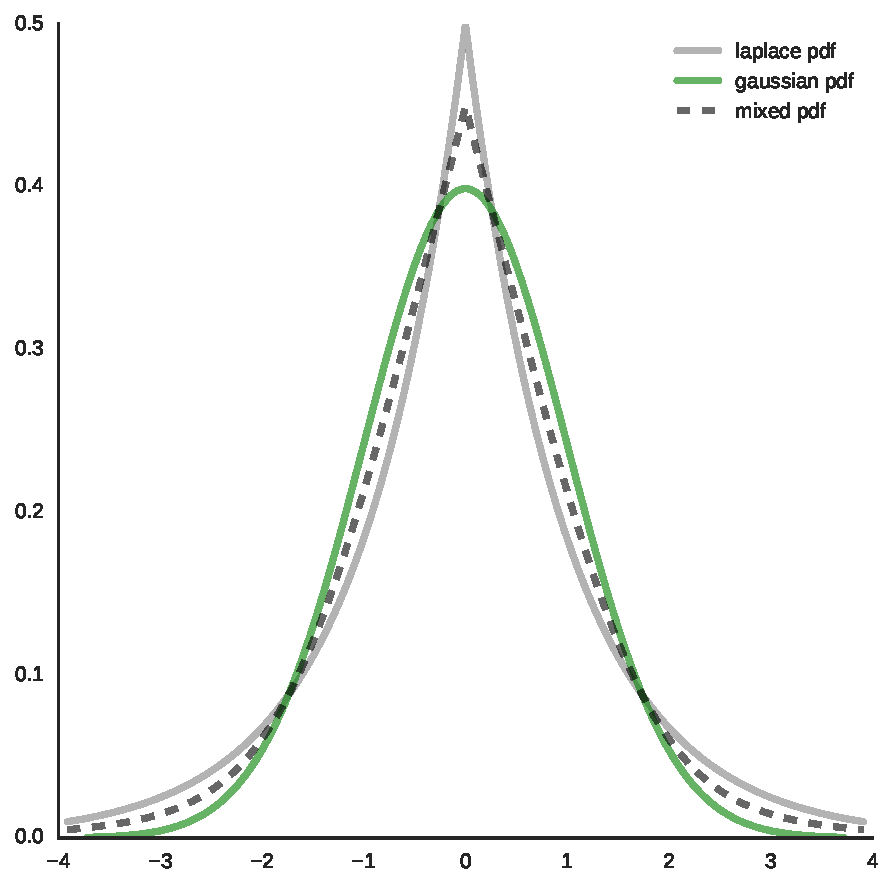
\includegraphics[width=0.7\textwidth]{pdfs}
    \caption{Plot of priors for ridge, lasso and elastic net.}\label{fig:reg-pdfs}
\end{figure}
\begin{figure}[tb]
    \centering
    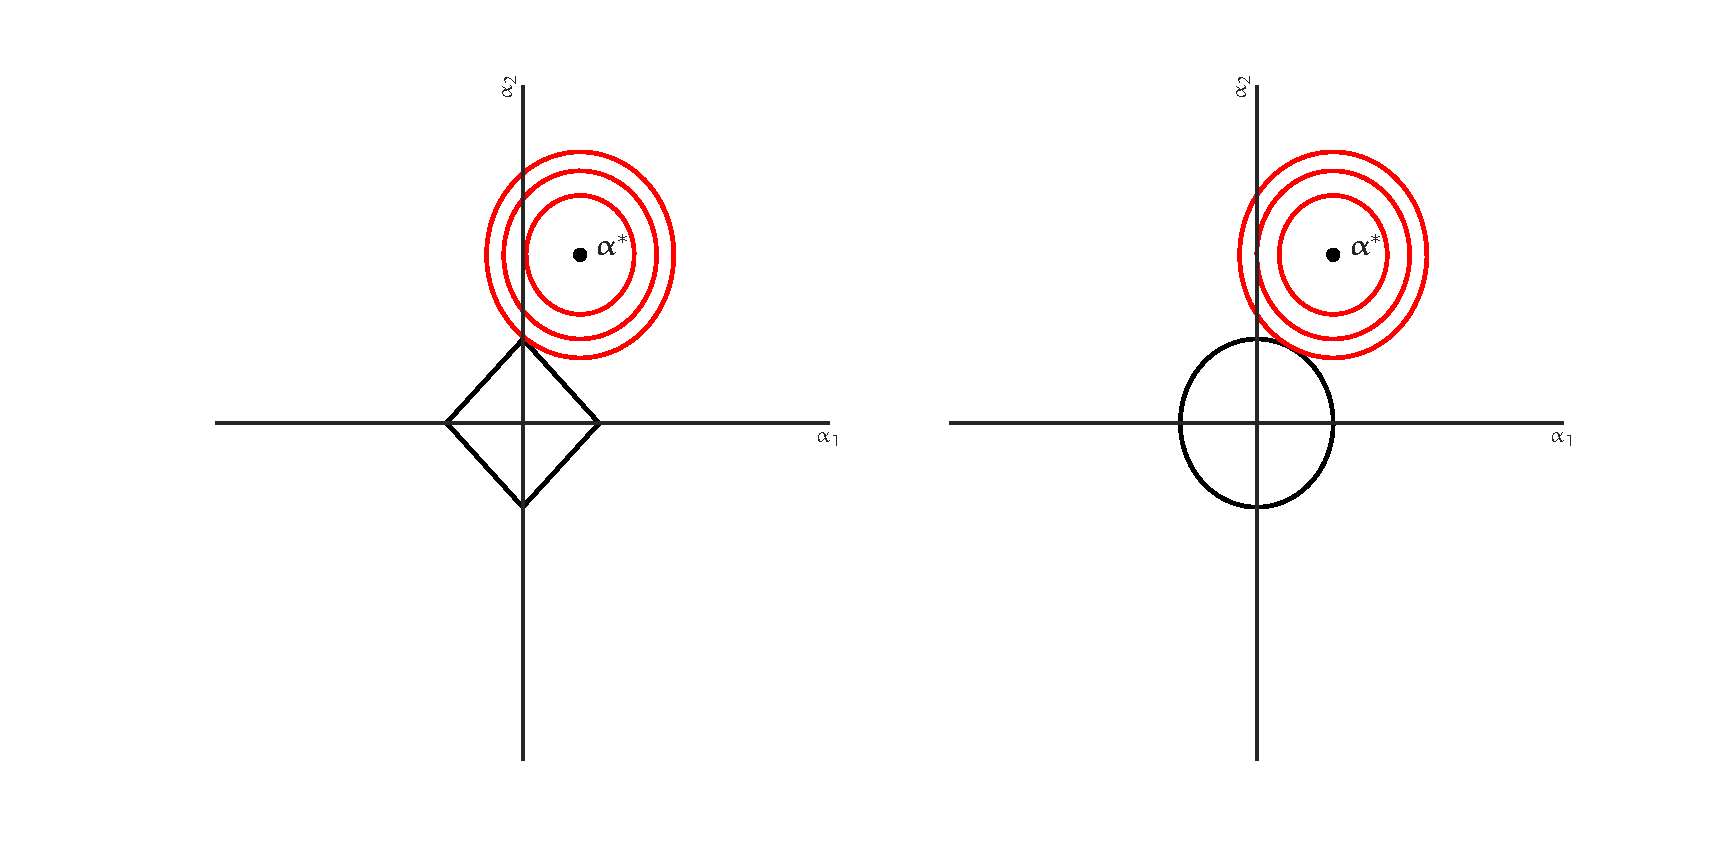
\includegraphics[width=0.7\textwidth]{constraints}
    \caption{Constraint regions}
\end{figure}

We can also view this smoothness function from a Bayesian perspective.
In this context lasso regularization can be seen as a Laplace prior on the
weights with zero mean.
A visualization of the prior can be seen in \cref{fig:reg-pdfs}.
We can see, that the Laplace prior puts more of its weight at zero and on its
tails than the normal distribution, which implies that solutions are more likely
to be exactly zero or larger than for the ridge estimate~\cite{lasso}.
The lasso is an instance of a special regularization functional family --- where
the penalty is realized as the \(l_p\) norm of the weights.
Fully beware of the notational abuse, we define the ``\(l_o\)-norm'' as the
cardinality of the support, i.e.~the number of entries of a vector that are not
zero.
The \(l_o\) penalty then corresponds to the standard best-subset
feature-selection.
It turn out, that the \(l_p\) norms are only convex for \(p \geq 1\).
The lasso can be therefore seen as the best convex approximation of the
best-subset method~\cite{sparse-learning,lasso}.

All perspectives show that the method results in sparse solutions --- 
solutions where one variable is exactly zero are more likely to occur for the
lasso functional.

\sidetitle{Elastic Net}
The lasso does not show good results in the following situations~\cite{elasticnet}:
\begin{itemize}
\item In the (\(n < p\))-case, the lasso selects at most \(n\) predictors.
\item When the predictors are highly correlated, the lasso selects one of the
  predictors at random, or shows otherwise unstable behaviour.
\item The Tikhonov regression shows better practical results than the lasso in the
  correlated case.
\end{itemize}
All those reasons indicate, that the lasso is not a good choice for some problems.
The Tikhonov regression is no direct competitor, because it does not lead to
sparse solutions.
We now discuss an alternative regularization methods, that is a combination of the lasso and the ridge penalties: the elastic net.
It was first introduced in~\cite{elasticnet} by \citeauthor{elasticnet}.

The elastic net functional is given by
\begin{equation}
  \label{eq:elastic-net}
  \lambda \mathcal{S}(\bm{\alpha}) = \lambda \Vert \bm{x} \Vert_2 +  \gamma \Vert \bm{x} \Vert _1,
\end{equation}
where \(\lambda\) and \(\gamma\) are two independent parameters~\cite{elasticnet}.
Although this form is more convenient for some following calculations, it is not intuitively useful for actual usage.
We can re-parametrize the previous equation as
\begin{equation*}
  \lambda_1 \mathcal{S}(\bm{\alpha}) = \lambda_1 \left( \left(1 - \lambda_2 \right) \Vert \bm{x} \Vert_2  + \lambda_2 \Vert \bm{x} \Vert _1\right),
\end{equation*}
where \(\lambda_1\) determines the overall regularization effect and \(\lambda_2\) controls the relative influence of the lasso term.
From this equation we can recover both the ridge and the lasso regularization, by setting \(\lambda_2\) to \(0\) or \(1\) respectively.
The ridge part of the penalty is able to overcome the limitations of the lasso
for correlated variables by shrinking them together~\cite{elasticnet}.

\sidetitle{Group Lasso}
Another useful generalization of the lasso is the grouped lasso that shrinks groups of weights at the same time.
Either all members of a group are selected, or none at all.
It was first developed by \citeauthor{grouplasso} in~\cite{grouplasso}, then
extended to the logistic regression method in~\cite{grouplasso-logistic}.
\citeauthor{grouplasso-generalizations} discussed some generalizations of the
method in~\cite{grouplasso-generalizations} and a discussion of the statistical
properties is offered by~\cite{grouplasso-benefit}.
The discussion here follows~\cite{sparse-learning}, unless otherwise noted.

Let \(\mathcal{P}\) denote a partition of \(\bm{\alpha}\), i.e.~a set of disjoint subsets whose union is \(\bm{\alpha}\).
We can then define the group lasso as
\begin{equation*}
  \mathcal{S}({\bm{\alpha}}) = \lambda \sum_{p \in \mathcal{P}} \left(\sqrt{\vert p \vert}\right) \Vert  p \Vert_2,
\end{equation*}
where \(\vert p \vert\) denotes the cardinality of \(p\) and is used as a weighting factor.
We can choose to weight the groups differently, but the square root of the
cardinality is a useful factor that is simple to calculate and which works well in practice.
If we would not include this factor, larger groups would be more likely to be included in the final model~\cite{sparse-learning}.

\sidetitle{Order of grid points}
Let
\begin{equation*}
  \operatorname{order}(\bm{p}) = \vert \{ i | p_i \neq 0.5 \} \vert
\end{equation*}
denote the cardinality of the support for a grid point with coordinates \(\bm{p}\).
A basis function with coordinate 0.5 for a dimension is constant in respect to
this dimension.
For example, the bias term is constant for all dimensions and has therefore
order zero.
The points of order one correspond to all basis functions that are constant for
all but one dimension, and so on.
We call all grid points with order larger than one interaction terms, because
they model the interaction between different dimensions.
We then partition our weights into groups consisting of all terms of the same order.
This grouping corresponds to the original predictors, including the interactions
between them.
\Cref{alg:group} shows a possible algorithm which results in our chosen
partition.
Note that we can recover the original lasso penalty by choosing partitions of size one.

\begin{algorithm}[h]
\caption{Group Lasso: Group}\label{alg:group} 
 \begin{algorithmic}[1]
   \Statex
   \Function{group}{gridStorage, $\bm{\alpha}$} 
    \Let{curGroup}{0}
    \Let{groups}{HashMap<vector<bool>, int>()}
    \Let{groupVec}{vector<bool>()}
    \For{point \(\in\) grid}
      \Let{usedDims}{vector<bool>(false,\ldots, false)}
      \For{\(\text{curDim} \in \{ 0, 1, \ldots, d\}\)}
        \Let{coordinate}{\Call{getCoordinate}{point, curDim}}
        \Let{usedDims[curDim]}{coordinate \(\neq\) 0.5}
      \EndFor
      \If{usedDims \(\in\) groups}
        \Let{groupVec[\Call{getSeqNumber}{point}]}{groups[usedDims]} 
        \Else
          \Let{groupVec[\Call{getSeqNumber}{point}]}{curGroup}
          \Let{curGroup}{curGroup + 1}
      \EndIf
    \EndFor
   \State \Return{groups, groupVec}
   \EndFunction
 \end{algorithmic}
 \end{algorithm}

It can be shown that the group lasso penalty performs better than the lasso
regularization, if the group structure is evident in the data.
If the structure is not contained in the data, the lasso method shows stronger
theoretical results.
For a more elaborate discussion of the theoretical performance of the group lasso, we refer to~\cite{grouplasso-benefit} by \citeauthor{grouplasso-benefit}.

The lasso functional --- and thus also the elastic net smoothness term --- is not differentiable at zero.
We were able to solve the Tikhonov regularization method using a standard conjugated gradient scheme, this is not possible for the methods presented in this section.
We cannot rely on gradient information any more, we need to solve this problem using a gradient-free optimization procedure.
This does not mean, that we have to use a black-box-optimization algorithm, we can still profit from the structure of our problem.
In the following section we present a solver for least-squares problems with
sparse regularization.

\subsection{Proximal Methods}
There are many solvers for the lasso and related methods.
In this section we present the Fast Iterative Shrinkage Tresholding Algorithm (\fista), first introduced in~\cite{fista}.
This solver offers a good compromise between flexibility and performance and we
can use it to solve all presented sparse regularization methods.
The discussion of \fista\ follows~\cite{fista}, the description of
the proximal operators follows~\cite{proxsurvey}.
\fista\ is able solve problems of the form
\begin{equation}\label{eq:composite-goal}
\min_{\bm{\alpha}} F(\bm{\alpha}) = f(\bm{\alpha}) + g(\bm{\alpha}),
\end{equation}
i.e.~minimizing functions that can be expressed as a sum of a convex, smooth function \(f(\bm{\alpha})\) and another convex, possibly non-smooth function \(g(\bm{\alpha})\).
\sidetitle{Lipschitz constant}
It is required that \(f(\bm{\alpha})\) has a Lipschitz-continuous gradient. 
This means that the following condition holds for all possible vectors \(\bm{x}\) and \(\bm{y}\) for some positive constant \(L\):
\begin{equation}   \label{eq:lipschitz}
 \Vert \bm{\nabla} f(\bm{x}) - \bm{\nabla} f(\bm{y}) \Vert \leq L \Vert \bm{x} - \bm{y} \Vert.
\end{equation}
We call the smallest possible value of \(L\) the Lipschitz constant.

For our goal given by \cref{eq:composite-goal} we set \(f(\bm{\alpha})\) to
\begin{equation*}
 f(\bm{\alpha}) = \frac{1}{2} \left\Vert  \bm{\Phi} \bm{\alpha} - \bm{y}   \right\Vert_2^2,
\end{equation*}
such that the gradient of \(f\) is then given by
\begin{equation*}
  \bm{\nabla} f(\bm{\alpha}) = \bm{\Phi}^\intercal \left(\bm{\Phi} \bm{\alpha} - \bm{y} \right).
\end{equation*}
The Lipschitz constant for the gradient of \(f\) is
\begin{equation}
  \label{eq:lipf}
  L_{\bm{\nabla} f} = {\left(\sigma_{\max} \left(\bm{\Phi}\right)\right)}^2,
\end{equation}
where \(\sigma_{\max} \) corresponds to the maximum singular value~\autocite{fista}.
Additionally we set \(g\) to
\begin{equation*}
  g(\bm{\alpha}, \lambda) = \mathcal{S} \left( \bm{\alpha}, \lambda \right).
\end{equation*}

\sidetitle{Moreau envelope}
We now define the Moreau envelope of a function \(g (\bm{\alpha})\), which is given for any \(\lambda \in (0, +\infty)\) by
\begin{equation}
  \label{eq:moreau-reg}
  M_{g}(\bm{\alpha}, \lambda) = \inf_{\bm{x}} \left\{  g(x) + (1/(2\lambda)) \Vert x - \bm{\alpha} \Vert_2^2 \right\}.
\end{equation}
It is a regularized, smooth version of our function \(g(\bm{\alpha})\) that has the
same minimum as \(g(\bm{\alpha})\).
That means, that every point that minimizes \(M_{g}(\bm{\alpha}, \lambda)\) also
minimizes our original function \(g (\bm{\alpha})\)~\cite{proxsurvey}.
Finally, we are able to define the proximal operator that returns the infimum
point of \cref{eq:moreau-reg} by
\begin{equation}
  \label{eq:proximal}
  \prox[\(g\)]{\bm{\alpha}}{\lambda}= \argmin_{\bm{x}} \left\{ g (\bm{x}) + (1/ (2 \lambda)) \Vert \bm{x} - \bm{\alpha} \Vert_2^2 \right\}.
\end{equation}
\sidetitle{Proximal Operator}
The proximal operator can be viewed as a gradient step with stepsize \(\lambda\) on the Moreau envelope
\(M_g(\bm{\alpha}, \lambda)\)
\begin{equation*}
  \prox[\(g\)]{\bm{\alpha}}{\lambda} = \bm{\alpha} - \lambda \bm{\nabla} M_{g}(\bm{\alpha}, \lambda).
\end{equation*}
This identity follows by rewriting \cref{eq:moreau-reg} in terms of the proximal operator and calculating the gradient~\cite{proxsurvey}.
We can use \cref{eq:proximal} to minimize \(M_g(\bm{\alpha}, \lambda)\) and
thus also for optimizing \(g(\bm{\alpha})\).
In the most general case \cref{eq:proximal} would imply the need to solve a convex optimization problem.
Fortunately we can find closed form solutions for many functions.
Consider for example \(g(\bm{\alpha}) = 0\).
In this case the Moreau envelope and the proximal operator are trivial
\begin{align*}
 M_{0}(\bm{\alpha}, \lambda) &= \inf_{\bm{x}} \left\{ 0 + 1/(2 \lambda) \Vert \bm{\alpha} - \bm{x} \Vert_2^2 \right\}, \\
 \prox[\(0\)]{\bm{\alpha}}{\lambda} &= \bm{\alpha}.
\end{align*}
It is obvious that the minimum of \(M_g(\bm{\alpha}, \lambda)\) is equivalent to the minimum of \(g(\bm{\alpha})\), the proximal operator is corresponds to a gradient step on \(M_g\).

We are now going to develop a minimizer for our composite goal that resembles a majorization-minimization algorithm.
To do this, we first define an upper-bound of \(F(\bm{\alpha})\)~(\emph{majorizing}) that we are then going to minimize~(\emph{minimization})~\autocite{proxsurvey}.

\sidetitle{Upper Bound}
We first give a regularized linearization of \(f(\bm{\alpha})\) at an arbitrary,
but fixed point \(\bm{y}\) for an \(L > 0\):
\begin{equation}\label{eq:f-approx}
  \hat{f}_L(\bm{\alpha}, \bm{y}) = f(\bm{y}) + \left< \bm{\alpha} - \bm{y}, \bm{\nabla} f (\bm{y}) \right> +
  L/2 \Vert \bm{\alpha} - \bm{y} \Vert_2^2,
\end{equation}
where the angle brackets \( \left< \bm{x}, \bm{y} \right> = \bm{y}^\intercal \bm{x} \) represent the inner product.
The first two summation terms are given by the first order Taylor expansion of \(f(\bm{\alpha})\) at the point \(\bm{y}\), the last term can be interpreted as a trust-region or regularization, that punishes large deviations from~\(\bm{y}\)~\cite{proxsurvey}.
We then combine this linearization with our second function to archive an upper-bound of \(F(\bm{\alpha})\):
\begin{equation}\label{eq:goal-approx}
  Q_L(\bm{\alpha}, \bm{y}) = f(\bm{y}) + \left< \bm{\alpha} - \bm{y}, \bm{\nabla} f (\bm{y}) \right> +
  L/2 \Vert \bm{\alpha} - \bm{y} \Vert_2^2 +
  g(\bm{\alpha}).
\end{equation}
We can see from \cref{eq:lipschitz} that \(Q_L(\bm{\alpha}, \bm{y})\) is an
upper-bound of \(F(\bm{\alpha})\) iff.~L is equal to or greater than the Lipschitz
constant of \(\bm{\nabla} f(\bm{\alpha})\).

\sidetitle{Fixed-point minimizer}
The minimizer for this approximation is then given as the fixed-point equation
\begin{align}\label{eq:step}
  \pi_{g(\bm{\alpha})}(\bm{\alpha}^*, L) &=  \argmin_{\bm{x}} \left\{ Q_L(\bm{x}, \bm{\alpha}) \right\}\nonumber\\
       &= \prox[\(g\)]{\bm{\alpha^*} - L^{-1} \bm{\nabla} f (\bm{\alpha^*})}{L^{-1} } \nonumber\\
       &= \prox[\(g\)]{\bm{\alpha^*} - L^{-1} \bm{\Phi}^\intercal \left(\bm{\Phi} \bm{\alpha^*} - \bm{y} \right)}
         {L^{-1}},
\end{align}
where \(\bm{\alpha}^*\) denotes the optimal solution and \(L\) is the Lipschitz constant of \(\bm{\nabla} f\) given by \cref{eq:lipf}~\cite{fista}.
In this equation \(L\) is used to determine the optimal stepsize.
This minimizer is called proximal gradient algorithm (or proximal-splitting) in the literature, because we first perform a gradient step on \(f'_L(\bm{\alpha})\) given by~\ref{eq:f-approx} and then a proximal step on \(g(\bm{\alpha})\)~\cite{proxsurvey}.
Using \cref{eq:step} repeatedly on a point will result in the fixed-point, i.e.~the minimum of the upper bound, and thus also in the minimum of our original goal~\cite{proxsurvey}.

\begin{algorithm}
 \caption{Iterative Shrinkage Tresholding Algorithm (\ista)~\cite{fista}}\label{alg:ista} 
 \begin{algorithmic}[1]
   \Require{Lipschitz constant \(L\) of \(\bm{\nabla} f\), regularization parameter \(\lambda\)}
    \Statex
    \Function{Ista}{$L, \bm{\alpha}$} \Comment{\(\bm{\alpha}\) is an initial guess}
      \While{not converged}
        \Let{$\bm{\alpha}$}{\( \pi_{g(\bm{\alpha})} \left( \bm{\alpha}, L \right) \)}
      \EndWhile
     \State \Return{\(\bm{\alpha}\)}
    \EndFunction
\end{algorithmic}
\end{algorithm}

\Cref{eq:step} is all we need to define the simple iterative scheme called
Iterative Shrinkage Tresholding Algorithm~(\ista) as seen in \cref{alg:ista}.
Originally the name \ista\ was only used for solving the Lasso problem, but is now used for the more general algorithm as well. 
For our trivial function \(g(\bm{\alpha}) = 0\) this iterative scheme is identical to the standard gradient descent algorithm.

\sidetitle{Proximal Operators for Regularization}
So far we have only seen the proximal operator of a very simple function.
This is of course not satisfactory, the motivation for this chapter is solving the Lasso and the Elastic Net regularization problems.
Fortunately, closed form solutions for the other needed proximal operators exist as well:
\begin{align}
\label{eq:prox-lasso}
\text{for Lasso} \quad &&
    \left( \prox[\(\lambda \Vert \bm{\alpha} \Vert_1\)]{\bm{\alpha}}{t} \right)_i &= \left[\alpha_i - t \lambda \right]_+
    - \left[ -\alpha_i - t \lambda \right]_+, \\
\text{for Ridge} \quad &&
                          \left(  \prox[\( \lambda \Vert \bm{\alpha} \Vert_2^2\)]{\bm{\alpha}}{t} \right)_i &= (\alpha_i/(1 + 2t \lambda)), \nonumber\\
  \text{for Elastic Net} \quad && \prox[\( \lambda \Vert \bm{\alpha} \Vert_1 + \gamma \Vert \bm{\alpha} \Vert_2^2\)]{\bm{\alpha}}{t} &=
                                                                                                                                       \left( 1/(1 + 2 t \gamma) \right) \left(\prox[\(\lambda \Vert \bm{\alpha} \Vert_1\)]{\bm{\alpha}}{t}\right) \nonumber\\
  \text{for Group Lasso} \quad && {\left(\prox[\( \lambda \sum_{p \in \mathcal{P}} \sqrt{\vert p \vert} \Vert p \Vert_2 \)]{\bm{\alpha}}{t} \right)}_p &=
                                                                                     \left[ 1 - \left(\lambda t \sqrt{\vert p \vert}\right) \left( \Vert p \Vert_2 \right)^{-1} \right]_+ p \nonumber
\end{align}
where \( \left( x \right)_+ = \max(x, 0) \) denotes the positive part of \(x\)
and \(t\) is a stepsize.
The regularization parameters depend on the function \(g(\bm{\alpha})\).
We omit the derivations for the sake of brevity, the interested reader refers to the survey paper~\cite{proxsurvey}.
By setting the regularization parameter \(\lambda\) equal to zero, we again recover the gradient minimization method.

\sidetitle{Minimizing Lasso}
These proximal operators can be used to define a minimizer for a non-smooth
function \(g\).
For example, combining~\cref{eq:step} with the proximal operator for the
Lasso functional \(g(\bm{\alpha}) = \lambda \Vert \bm{\alpha} \Vert_1\) given by~\cref{eq:prox-lasso} results in
the minimizer
\begin{align*}
  \pi_{\lambda \Vert \bm{\alpha} \Vert_1}(\bm{\alpha^*} ,L)
  &=  \prox[\(\lambda \Vert \bm{\alpha} \Vert_1\)]{\bm{\alpha^*} - L^{-1} \bm{\nabla} f (\bm{\alpha^*})}{L^{-1}} \\
  &= {\left[ \left(\bm{\alpha^*} - L^{-1} \bm{\nabla} f (\bm{\alpha^*}) \right) - \lambda L^{-1} \right]}_+ -
    {\left[ -\left(\bm{\alpha^*} - L^{-1} \bm{\nabla} f (\bm{\alpha^*}) \right) - \lambda L^{-1} \right]}_+,
\end{align*}
again given as a fixed-point iteration.
In this equation the function \( \left[ x \right]_+ \) is applied element-wise on its input vector.
We can then use this minimizer with \cref{alg:ista} to compute a solution to
the Lasso problem.
The fixed-point equations for the Lasso and Elastic Net Regularization are
computed analogously.

\sidetitle{Nesterov's accelerated gradient descent}
\ista always converges to the global maximum, but only does so linearly~\cite{fista}.
To overcome this problem, Beck and Teboulle combined the \ista algorithm with
the accelerated gradient descent algorithm discovered by Nesterov. 
Nesterov's accelerated gradient descent is closely related to the ordinary
gradient descent algorithm.
The first step is identical, each following step carries some momentum of the
step before, thus stabilizing the procedure.
It is an optimal first-order optimization schema, i.e.~one that cannot be
improved asymptotically.
It archives quadratic convergence.
This property is retained when combined with the proximal-splitting procedure \cref{alg:ista}, the result is called \fista~\cite{fista}.
Each step of \fista\ evaluates the gradient and the proximal operator once, just as \ista does.
This means that the accelerated algorithm has a comparable cost for each iteration.

\sidetitle{Linesearch}
Another problem with \cref{alg:ista} is its dependence on the Lipschitz constant of
\(\bm{\nabla} f\) to determine the optimal stepsize.
For our choice of \(f\), the best constant \(L\) is given by~\cref{eq:lipf}.
To avoid this expensive calculation, we use a backtracking line search to
determine a suitable stepsize.
In this line search procedure we use \cref{eq:goal-approx} as an upper bound for \cref{eq:composite-goal}.
We do this by iterating and finding the smallest \(L\) for which
\cref{eq:goal-approx} is an upper bound.
This always results in the Lipschitz constant~\cite{fista}.
It is then straightforward to derive \cref{alg:linesearch}.

\begin{algorithm}[h!]
 \caption{Linesearch~\cite{fista}}\label{alg:linesearch}
 \begin{algorithmic}[1]
  \Require{\(L > 0, \eta > 1, \bm{\alpha}\)} 
  \Statex
  \Function{Linesearch}{$\bm{\alpha}, L$}
    \Let{\(i\)}{\(0\)}
    \Do
      \Let{L}{\(\eta^i L\)}
      \Let{prox}{\(\pi_{\bm{\alpha}} (\bm{\alpha}, L)\)}
      \Let{\(i\)}{\(i + 1\)}
    \doWhile{$F(\text{prox}) < Q_L(\text{prox}, \bm{\alpha})$}
    \State \Return{prox and \(L\)} \Comment{Also return prox to avoid duplicate calculations.}
  \EndFunction
 \end{algorithmic}
\end{algorithm}

We need to evaluate the line search once for each iteration step.
It is possible that this procedure finds a non-optimal \(L\), i.e.~an \(L\) that
is larger than the Lipschitz constant.
This leads to a smaller stepsize, which is not a problem in practice, because
our optimization procedure still converges, although slower than possible.
We have to take that into consideration for our choice of linesearch parameters.
Usual values are \(L = 0.5\) and~\(\eta = 2\).
Using \cref{alg:linesearch} we can finally present an optimal first order optimization algorithm, shown by \cref{alg:fista}.

It is of course possible to use a constant stepsize like in \cref{alg:ista}.
To do this, replace the line search with the minimal value of \(L\) and
calculate \(\pi(\bm{\alpha}, L)\) directly.
We can also integrate the linesearch into the \ista algorithm, by replacing the
fixed \(L\) with a call to the linesearch subroutine.
A comparison of the practical speed of \ista and \fista with constant stepsize can be seen in~\cref{fig:fista-convergence}.

An alternative backtracking scheme for \fista is offered in~\cite{fista-backtracking}.
It offers the same asymptotic convergence speed, but shows practical improvements for some minimization problems.

\begin{figure}[bt]
  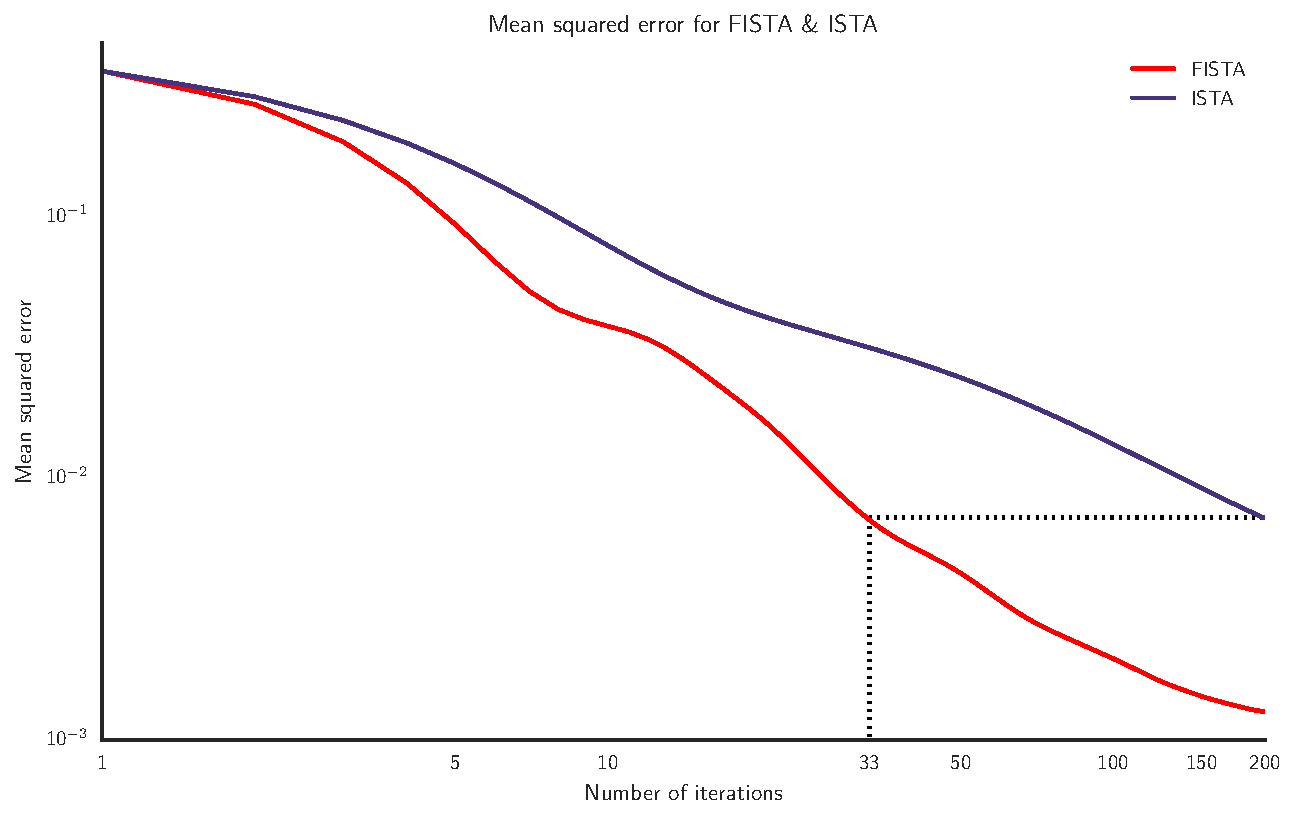
\includegraphics[width=\textwidth]{fista}
  \caption[Comparison of \fista and \ista]{Comparison of \fista and \ista, both with constant stepsize.
    The figure shows the training \textsc{mse} for 500
    iterations with \(\lambda = 0.1\) for the training set of the concrete
    data set.
    The dotted lines indicate the best value reached by \ista.
    Note that \fista is able to return a better result after only 56
    iterations ---
    compared to the 500 needed by \ista.
  }\label{fig:fista-convergence}
\end{figure}

\begin{algorithm}[h]
 \caption{Fast Iterative Shrinkage Tresholding Algorithm (\fista)~\cite{fista}}\label{alg:fista} 
 \begin{algorithmic}[1]
   \Require{Initial guess for Lipschitz constant \(L\) of \(\bm{\nabla} f\), regularization parameter \(\lambda\)}
    \Statex
    \Function{Fista}{$L, \bm{\alpha}$} \Comment{\(\bm{\alpha}\) is an initial
      guess for \(\alpha^*\).}
      \Let{\(\bm{y}\)}{\(\bm{\alpha}\)}
      \Let{\(t\)}{\(1\)}
      \While{not converged}
        \Let{\(\bm{\alpha}_{\text{before}} \)}{\(\bm{\alpha}\)}
        \Let{$\bm{\alpha}, L$}{\Call{Linesearch}{$ \bm{y}, L$ }} \Comment{Linesearch returns \(\pi_L (\bm{y})\) and the used L.}
        \Let{\(t_\text{before}\)}{\(t\)}
        \Let{\(t\)}{\(\nicefrac{1}{2} (1 + \sqrt{1+4t^2}) \)}
        \Let{\(\bm{y}\)}{\(\bm{\alpha} + \left( t_\text{before} -1 \right) t^{-1} 
                    \left(\bm{\alpha} - \bm{\alpha}_{\text{before}} \right)\)}
      \EndWhile
     \State \Return{\(\bm{\alpha}\)}
    \EndFunction
\end{algorithmic}
\end{algorithm}

%%% Local Variables:
%%% mode: latex
%%% TeX-master: "../main"
%%% End:


\section{Implementation}

\tikzumlset{fill class = white, fill template = white, fill package = white}

\begin{figure}[h]
  %https://tex.stackexchange.com/questions/140739/extending-figures-into-the-margin-on-even-vs-odd-pages
  \centering
 \makebox[0.9\textwidth][c]{\begin{tikzpicture}
    \begin{umlpackage}{RegularizationFunctions}
      \umlclass[type=abstact, x=1]{RegularizationFunction}{
      }{
        \umlvirt{+ eval(weights : DataVector) : double}\\
        \umlvirt{+ prox(weights : DataVector, stepsize : double) : DataVector}
      }

      \umlclass[y=0, x=10]{ZeroFunction}{}{
        + ZeroFunction()
      }

      \umlclass[y=6, x=0]{RidgeFunction}{
        - lambda : double
      }{
       + RidgeFunction(lambda : double)}

      \umlclass[y=-4, x=0]{LassoFunction}{
        - lambda : double
      }{
      + LassoFunction(lambda : double)}

      \umlclass[y=-4, x=10]{ElasticNetFunction}{
        - lassoFunc : LassoFunction \\
        - lambda1 : double\\
        - lambda2 : double
      }{
        + ElasticNetFunction(lambda : double, l1Ratio : double)
      }

      \umlclass[y=5, x=10]{GroupLassoFunction}{
        - lambda : double\\
        - groups : map<coords, int>\\
        - storage : gridStorage*\\
        - groupIx : map<int, index>\\
        - lastSize: int
      }{
        + GroupLassoFunction(lambda : double,\\
        \phantom{+ } storage : GridStorage*)\\
        - calculateNorm(weights : DataVector) : DataVector\\
        - calculateIndices(weights : DataVector) : void
      }

    \umlinherit[]{ZeroFunction}{RegularizationFunction} 
    \umlinherit[]{RidgeFunction}{RegularizationFunction} 
    \umlinherit[]{LassoFunction}{RegularizationFunction} 
    \umlinherit[]{ElasticNetFunction}{RegularizationFunction} 
    \umlinherit[]{GroupLassoFunction}{RegularizationFunction} 

    \umlassoc{LassoFunction}{ElasticNetFunction}
    \end{umlpackage}
  \end{tikzpicture}}
  \caption[Class diagram for RegularizationFunctions]{Implementation of
    RegularizationFunctions}
\label{fig:uml-regularization-functions}
\end{figure}

\newcommand{\fistalb}{\\\phantom{+ solve(}}
\begin{figure}[htb]
\begin{tikzpicture}
  \begin{umlpackage}[x=0, y=0]{Fista}
    \umlclass[type=abstact, width=20ex]{sgpp::solver::FistaBase}{
      
    }{
        % + solve(op : OperationMultipleEval, \\\phantom{+ solve} weights : DataVector,
        % y : DataVector,\\\phantom{+ solve} maxIt : size\_t, threshold : double) : void
      \umlvirt{\parbox[c]{0.7\textwidth}{+ solve(op : OperationMultipleEval,
          \fistalb weights : DataVector,
        y : DataVector, maxIt : size\_t, \fistalb threshold : double, L : double) : void}}

    }

    \umlclass[template={F}, y=-4, name=Fista]{sgpp::solver::Fista}{
    - regularizationFunction : F 
    }{
      + Fista( regularizationFunction : F)\\
    }
       
    \umlinherit[]{sgpp::solver::FistaBase}{sgpp::solver::Fista}
  \end{umlpackage}
\end{tikzpicture}
\end{figure}

As seen in \cref{fig:uml-regularization-functions} we define a base class
RegularizationFunction, that offers the two methods eval and prox, that
calculate \(g(\bm{\alpha})\) and its proximal operator respectively.
Every parameter that is needed for each functional is passed during
construction, this way we archive a great amount of flexibility.
Classes that use the regularization functions do not have to be concerned about
the definition or the parameters of the functionals, they can treat them as a
black box.
We offer an implementation of the ridge, the lasso, the elastic net and the
group lasso function, that resemble the definitions outlined in this chapter.
The group lasso function uses the following subroutines:
\begin{description}
\item[calculateIndices] that partitions our weights into groups that share the
  same order. This method is only called when the grid size changes, so only
  once during the first solver iteration. When the grid size changes, e.g.~due
  to an adaptivity process, the groups are automatically recalculated. This is
  in contrast to the
\item[calculateNorm] method, that is called once per evaluation of the proximal
  operator, which calculates the group norms and the group size.
\end{description}
The ElasticNetFunction uses the LassoFunction to calculate the  \(l_1\) part of its evaluation.
Additionally we implemented a ZeroFunction, that can be used, when no
regularization is desired.

Our solver \fista is then implemented as a class with one template argument: the
proximal operator.
We therefore have to first create a RegularizationFunction and then a Fista
class.
Even though this might seem inconvenient, it allows the compiler to inline all
calls to both the function evaluation and the proximal operator, which get
called once in each loop.
Notice in the class diagram ???, we defined a base class FistaBase, that allows us to hold a pointer not only to a specalised Fista object, but also to one where we do not know the used RegularizationFunction.

\fista itself is split into various subroutines, that allow a separation of
concerns.
This leads to a very clean implementation, that closely represents
\cref{alg:fista}.
All call to the subroutines were inlined automatically, at least for the used
\emph{gcc}-compiler with the highest optimization settings.


As seen in the class diagram above, \fista is implemented as a templated class
that determines the used function \(g\).
The template allows the compiler to inline all calls to prox and eval, which get
evaluated once during each iteration.
Even though the implementation of \fista is split into various subroutines, they
all get inlined into one efficient loop.
We have to use a base class, otherwise we would not be able to attain a pointer
to the Fista class, without knowing the used type of regularization.
\FloatBarrier{}
\subsection{Results \textit{\&} Discussion}
We can calculate the value of \(\lambda\) for which all weights are exactly
zero, using the method developed by \citeauthor{regularizationpaths} in~\cite{regularizationpaths}.
The maximum \(\lambda\) is given by
\begin{equation*}
  \lambda_{\text{max}} = \frac{\max_i \vert \langle \bm{\Phi}_i, \bm{y} \rangle \vert}{\lambda_2 n},
\end{equation*}
where the index \(i\) denotes the \(i\)th column of the matrix, and
\(\lambda_2\) the amount of \(l_1\) regularization.
We then construct a logarithmic grid starting with \(\lambda_{\text{max}}\) to
\(\lambda_{\text{min}} = \varepsilon \lambda_{\text{max}}\), where
\(\varepsilon\) is typically set to 0.001.
It is more efficient to start the path with all weights set to zero, see~\cite{regularizationpaths} for a more advanced discussion.

We introduce our first dataset, the Friedman1 dataset, first published
in~\cite{datasets-friedman}.
Let \(\bm{x}^F = (x_1, \ldots, x_{10}) \in \mathbb{R}^{10}\) be a uniformly distributed vector.
We use \(\bm{x}\) as our predictors, and define
\begin{equation}\label{eq:friedman1}
  y = 10 \sin(\pi x_1 x_2) + 20(x_3 - 0.5)^2 + 10x_4 + 5x_5 + \varepsilon,
\end{equation}
with \(\varepsilon \sim \mathcal{N}(0,1)\) as additional Gaussian noise.
We perform some preprocessing steps on this dataset, these can be found in \cref{sec:friedman}.
This dataset has many useful properties, we will use it throughout this thesis.
The fact that the optimal error is given by the normal noise variance is
helpful, to determine the performance of this method.

We then calculated regularization paths for the lasso, the elastic net (with
\(\lambda_2 = 0.3\)) and the group lasso using an estimator with level 2 and the
Friedman1 dataset.
Those can be seen in figure xxx.
The elastic net method selects all terms at the same \(\lambda\) and then
applies shrinkage to all weights, which keeps them small.
The lasso on the other hand selects only the bias and then all other terms
one-by-one.
We can see that the lasso selects grid points that belong to the same
interaction at different times.
In contrast to that, the group lasso results in weights, where either all terms
of a group are selected, or none at all.

Using the same method we calculated the regularization paths for the lasso and
the grouped lasso again for the Friedman1 dataset, but this time using a level
three estimator.
The results are depicted in \vref{fig:friedman1-heatmap}.
We can see, that while the group norms are similar, the grid point selection of
the group lasso is more stable and selects points on a group level.

\begin{figure}[htb]
  \centering
  \begin{subfigure}[b]{\textwidth}
    \centering
    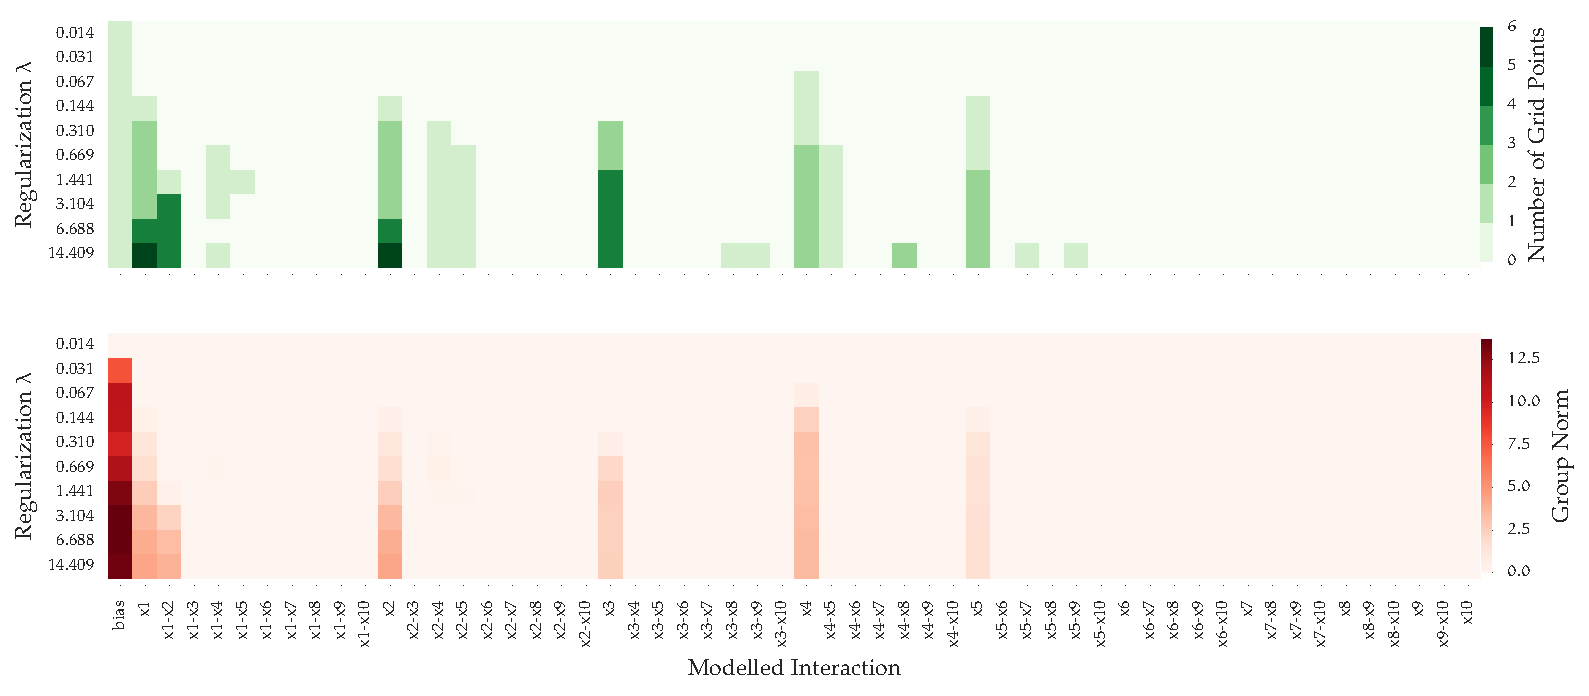
\includegraphics[width=\textwidth]{heatmap_lasso}
    \caption{Lasso}
  \end{subfigure}
  \begin{subfigure}[b]{\textwidth}
    \centering
    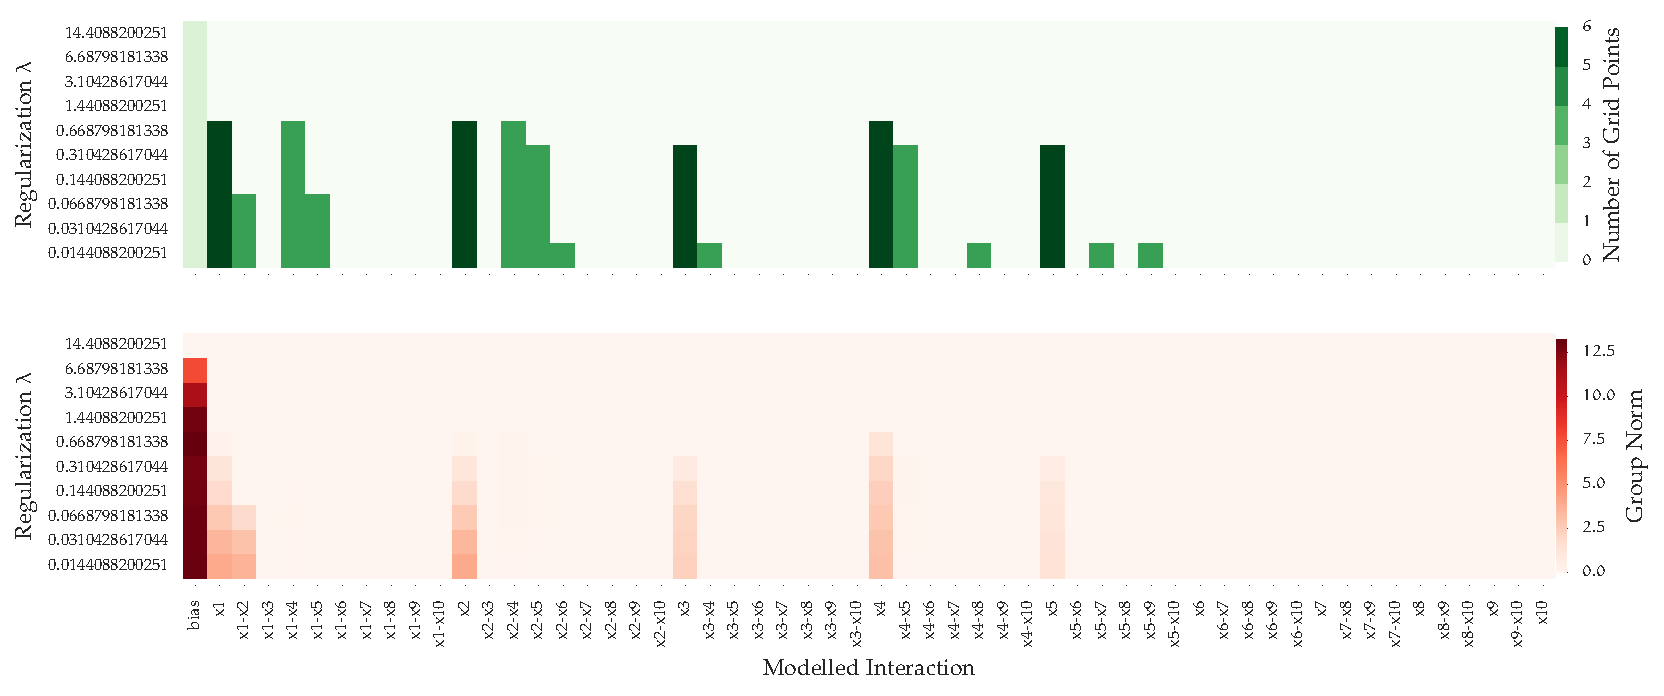
\includegraphics[width=\textwidth]{heatmap_grp}
    \caption{Group Lasso}
  \end{subfigure}
  \caption{Comparison of lasso and group lasso for the Friedman1 dataset with
  level 3.
  The x-axis corresponds to the modelled group and the y-axis to the regularization
  parameter \(\lambda\). Each figure shows two heatmaps. The first one shows
  the number of selected terms, the second one presents the \(l_2\) norm of the
  group terms.}\label{fig:friedman1-heatmap}
\end{figure}

We also performed a small grid search for the concrete dataset, using estimators
of level three and four.
Values of \(\lambda \in (10^{-1}, 10^{-2}, \ldots, 10^{-9})\) were tested.

We can see, that all regularization methods managed to perform well for a
large grid that has roughly five times more grid points than data points.
The performance archived was better than the best results for both tested
Tikhonov regularization methods.

%%% Local Variables:
%%% mode: latex
%%% TeX-master: "../main"
%%% End:

